\documentclass[letterpaper, 12pt]{article}

% Set Margins
\usepackage[margin=1in, includefoot]{geometry}

% Empty Bullets
\usepackage{enumitem}

% Set Images Path
\usepackage{graphicx}
\graphicspath{{./images/}}

% Allow Image Wrapping
\usepackage{wrapfig}

% Allow Floating Images
\usepackage{float}

% Use URLs
\usepackage{hyperref}
\hypersetup{
    colorlinks=true,
    linkcolor=black,
    filecolor=magenta,
    urlcolor=blue,
}

% Set Headers
\usepackage{fancyhdr}
\pagestyle{fancy}
\fancyhead{}
\fancyfoot{}
\fancyfoot[R]{\thepage}
\renewcommand{\headrulewidth}{0px}

\begin{document}

\begin{titlepage}
\begin{center}

\includegraphics[scale=0.35]{title}

\vspace{0.5in}

\textsc{\huge{ORCAH - Changed Up}}

\end{center}
\end{titlepage}

\section{Introduction}

Online Robotics Competition at-Home (ORCAH) is a student-led organization hosting unofficial scrimmages coming up to VEX Worlds 2021.  Our aim is to provide world-qualified teams the experience and resources they require to excel during these unprecedented times.  Through our free practice scrimmages leading up to our championship scrimmage, teams will be able to simulate and practice for Worlds, collaborate, and learn this new form of competition on a larger scale than prior events.

\subsection{Game Description}

Matches are played on a field setup as illustrated in the image below, with Red and Blue Alliance having mirrored field layouts and competing virtually.  This game was not originally designed to be played virtually, and we, ORCAH, have modified the points in the game slightly to make a more enjoyable experience for competitors and spectators.  The object of the game is to attain a higher score than the opposing Alliance by Scoring Balls and Connecting Rows.  

An Autonomous Win Point is awarded to any Alliance that completed a Connected Row using their Alliance Home Row at the end of the Autonomous Period.  

A point bonus is awarded to the Alliance that has the most points at the end of the Autonomous Period. 

With our new game rules comes a modified field layout.  Our field layout is asymmetrical with the side that you start similar to VEX’s field layout.  The goal of this is to not force teams to make new autonomous routines for their robots.

\begin{center}
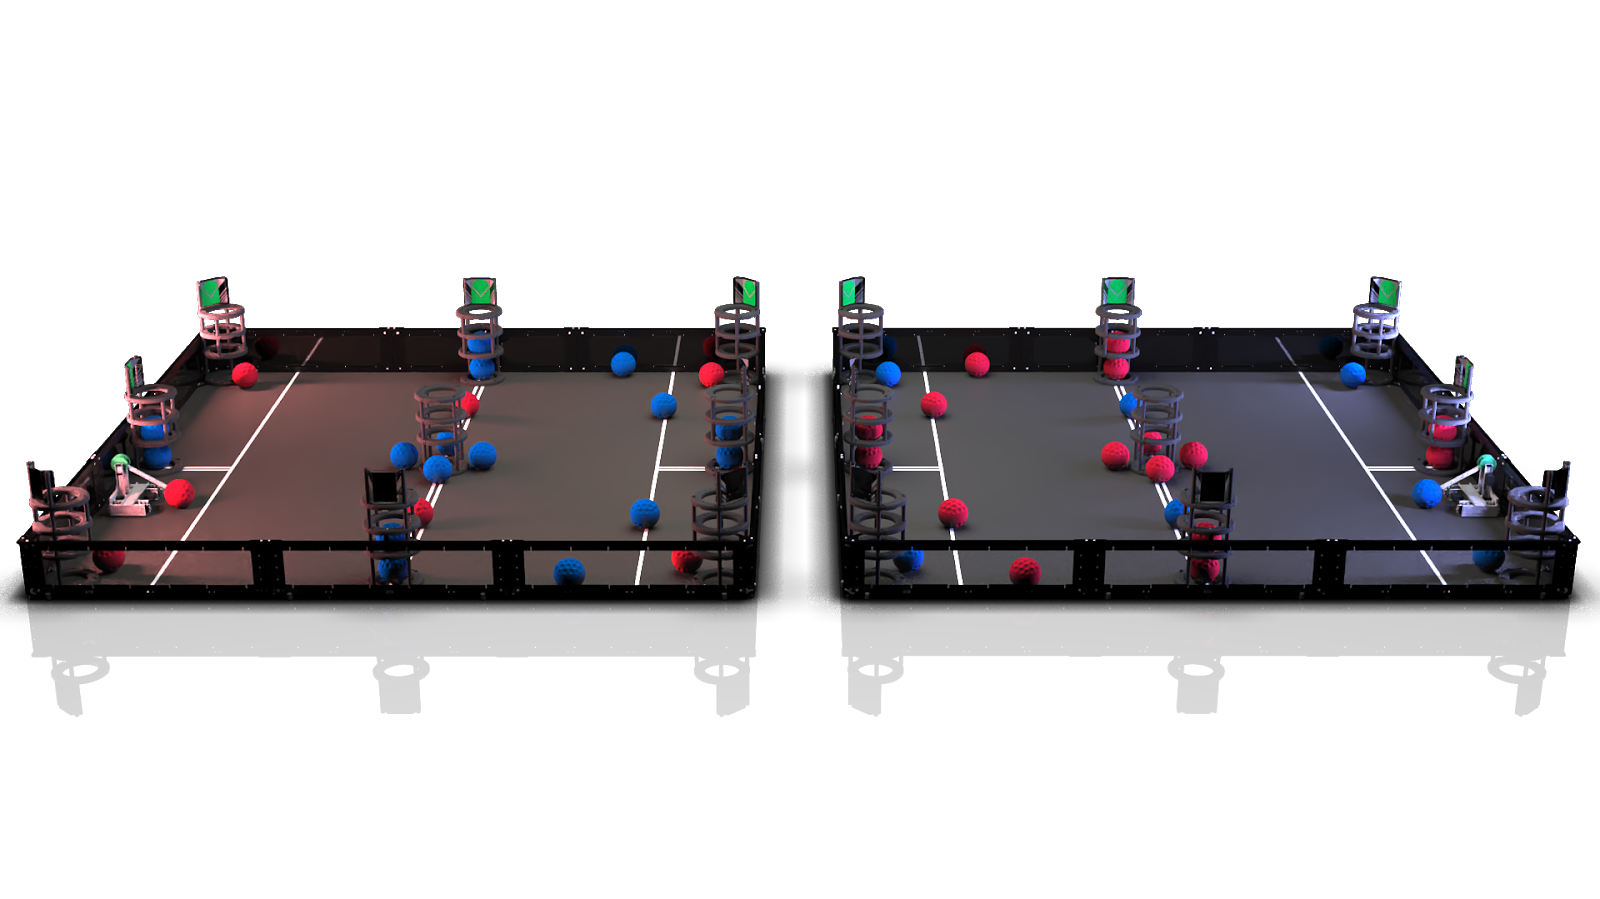
\includegraphics[scale=0.25]{fields}
\end{center}

\newpage

\section{The Game}
\subsection{Definitions}

\begin{itemize}[label={}]

\item\textbf{1 Point Ball} - Ball of your opponent’s Alliance color.

\item\textbf{2 Point Ball} - Ball of your Alliance color.

\item\textbf{Connected Row} - A Row where all three (3) Goals in the Row are Owned by the same Alliance.

\item\textbf{Outer Row} - The four (4) Rows that do not pass through the center Goal (Goal ‘E’).

\item\textbf{Center Row} - The four (4) Rows that pass through the center Goal.

\item\textbf{ORCAH Q\&A} - \href{https://sites.google.com/view/orcah-robotics/qa?authuser=0}{The Q\&A found here.}

\item\textbf{ORCAH Game Manual} - The document you are reading.

\item\textbf{REC Foundation Q\&A} - \href{https://www.robotevents.com/VRC/2020-2021/QA}{The Q\&A found here.}

\item\textbf{VEX Game Manual} - \href{https://content.vexrobotics.com/docs/vrc-change-up/Game-Manual-12012020.pdf}{The VEX Change Up game manual, found here.}

\item\textbf{Scored} - A ball is considered “Scored” if the ball is:

\begin{itemize}
\item[--] Fully or partially within the outer edge of the Goal.
\item[--] Fully below the upper edge of the Goal.
\item[--] Not contacting any foam tiles outside the Goal.
\end{itemize}

In the event that more than three Balls are scored in a Goal, the highest point combination of three (3) Balls will be Scored.

\item\textbf{Owned} - Similar to Live Remote Tournaments, Goal Ownership is determined by how many points are in the Goal. Goal Ownership is denoted by which color has the highest point total in a goal. Four (4) points in a goal Scored for red and three (3) points scored for blue would mean that the Goal is Owned by red.

\newpage

\item\textbf{Red Alliance Field} - The Red Alliance and Blue Alliance have mirrored field layouts to avoid requiring teams to recreate their autonomous functions for ORCAH’s game.  For virtual matches, the Red Alliance will be on the left side of the field from the audience point of view.

\begin{center}
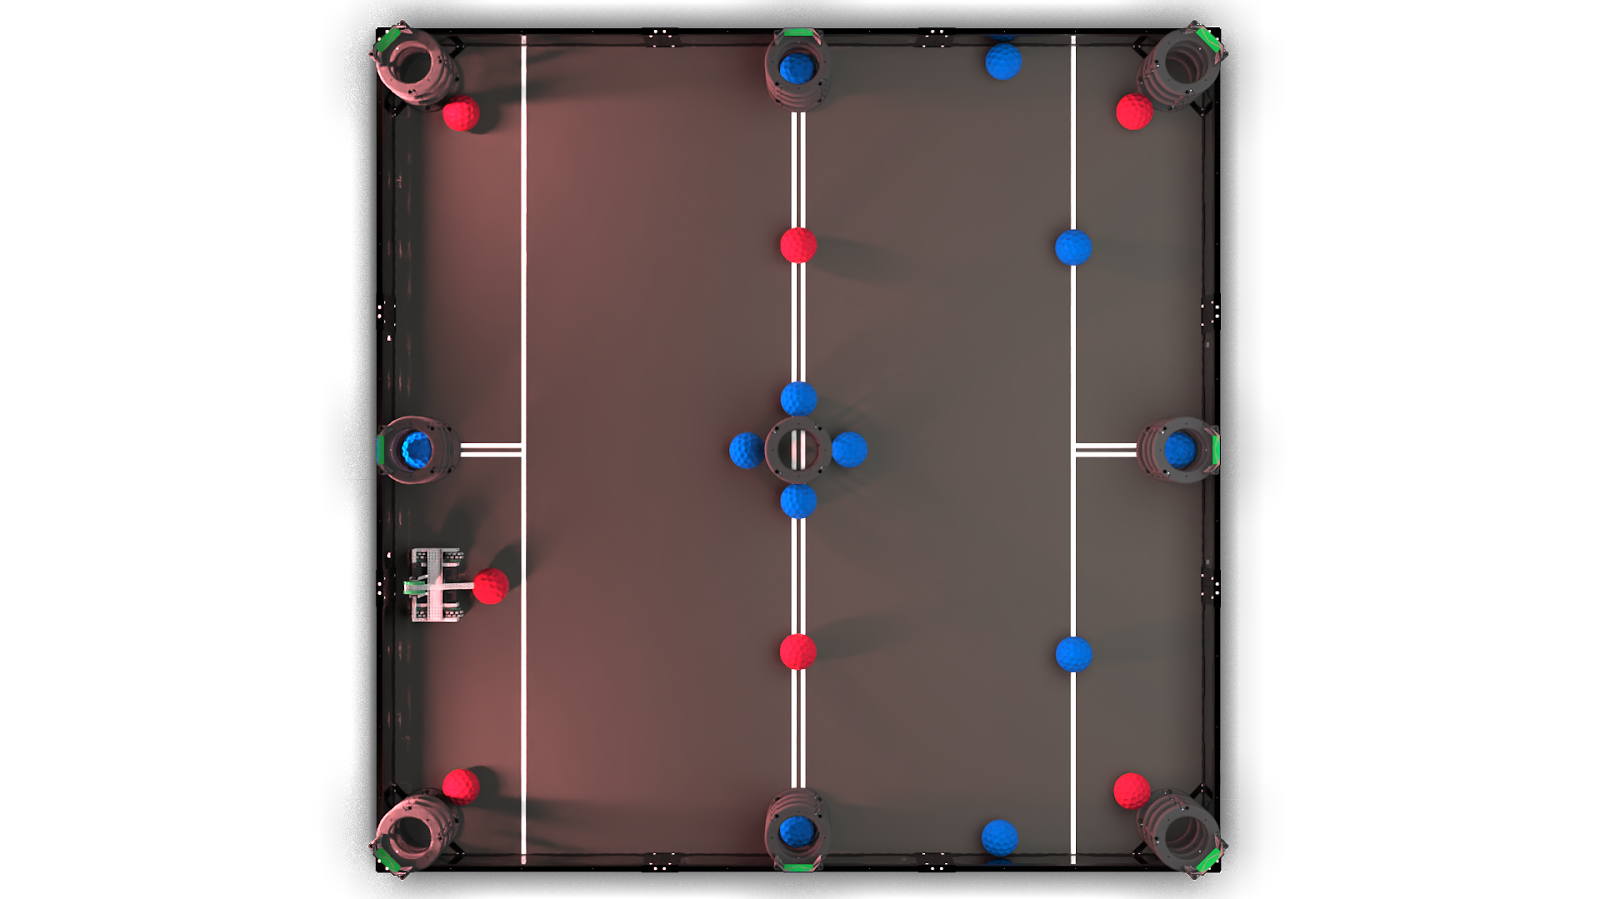
\includegraphics[scale=0.25]{redfield}
\end{center}

\item\textbf{Blue Alliance Field} - The Blue Alliance and Red Alliance have mirrored field layouts to avoid requiring teams to recreate their autonomous functions for ORCAH’s game.  For virtual matches, the Blue Alliance will be on the right side of the field from the audience point of view. 

\begin{center}
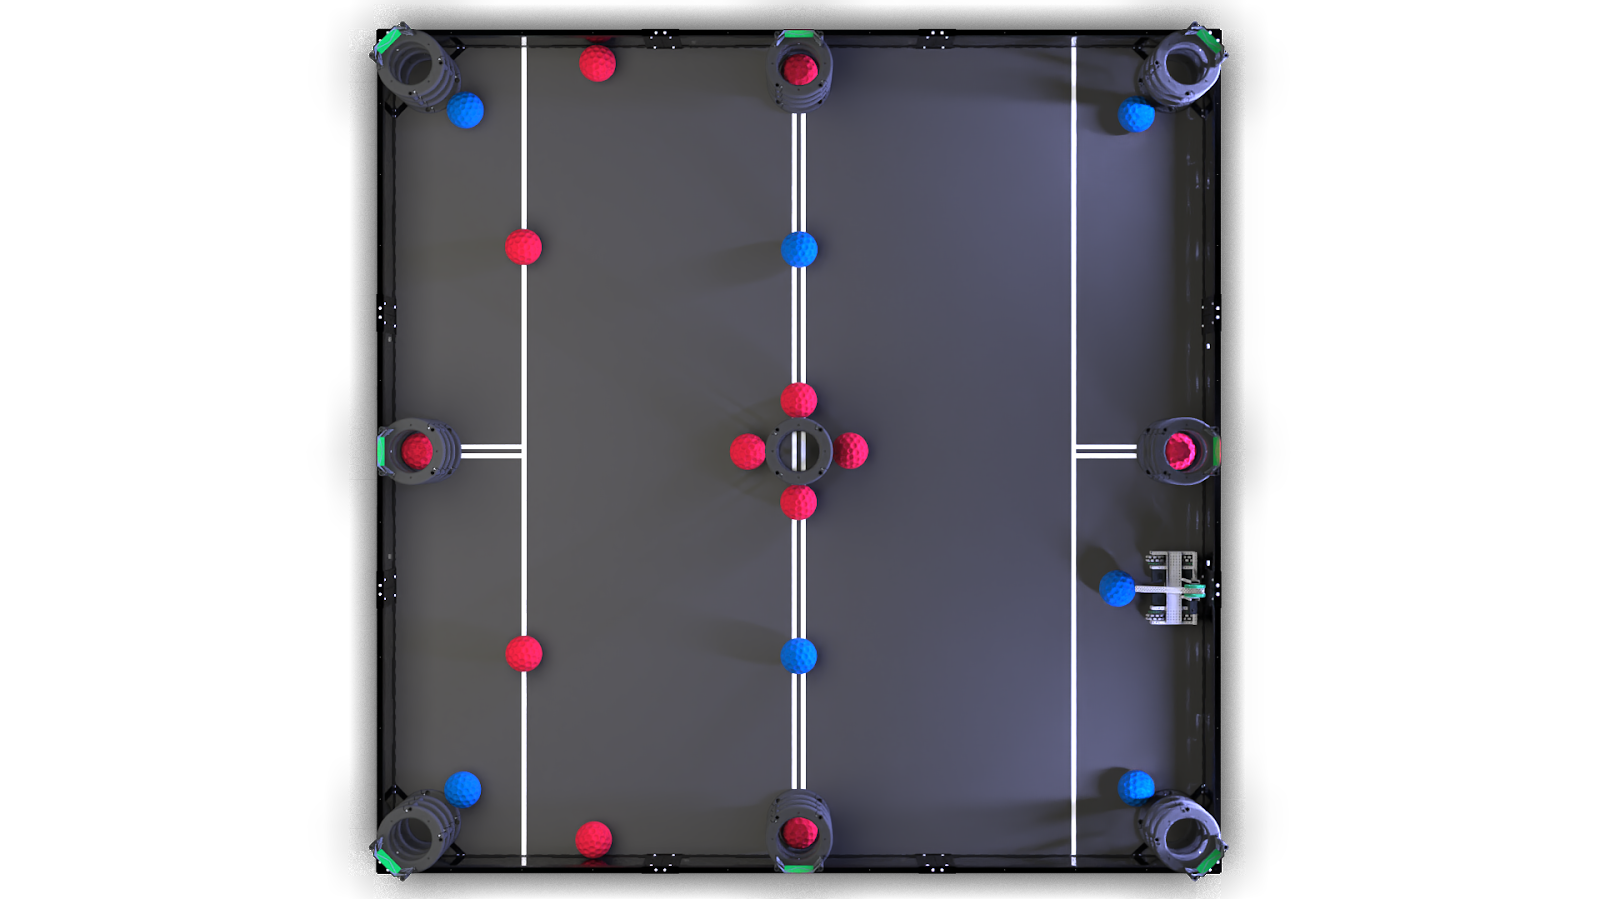
\includegraphics[scale=0.25]{bluefield}
\end{center}

\item\textbf{Goal Label} - To aid in remote communication and scoring, each Goal has a Goal Label, as shown in Figure 17. These Goal Labels are laid out relative to the Alliance Stations and audience view, and should be consistent between all four Team fields. For example, if a Head Referee were to ask Team members to “point at Goal A”, all Team members should point to the Goal in the top-left corner of the remote webcam feed.

\begin{center}
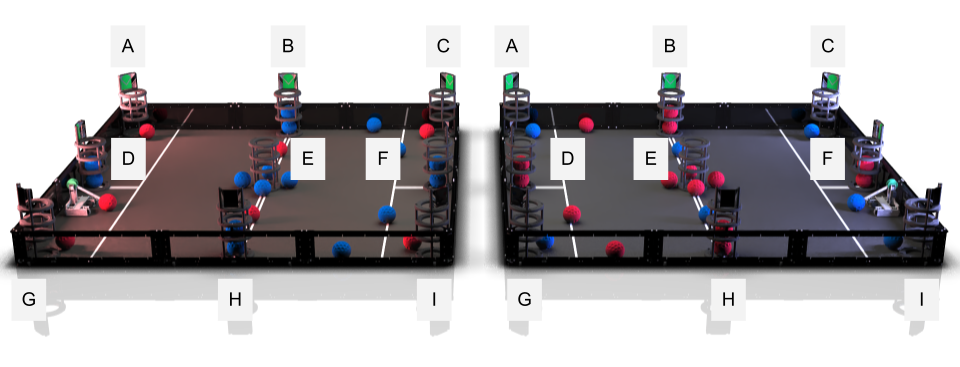
\includegraphics[scale=0.5]{labels}
\end{center}

\end{itemize}

\section{Game Manual Priority}

The order of priority is as follows:
\begin{itemize}
\item[--] ORCAH Q\&A
\item[--] ORCAH Game Manual
\item[--] REC Foundation Q\&A
\item[--] VEX Game Manual
\end{itemize}

For example, Scored is defined in the VEX Game Manual.  Scored is clarified in the REC Foundation Q\&A.  Scored is also defined in the ORCAH Game Manual.  If that is the most recent definition of Scored, then that is the official precedent.  If the ORCAH Q\&A clarifies it further, then that is the official precedent.

\section{Scoring}
\begin{itemize}
\item[--] Each Center Row is worth four (4) points for that Alliance.
\item[--] Each Outer Row is worth six (6) points for that Alliance.
\item[--] 2 Point Balls are worth two (2) points.
\item[--] 1 Point Balls are worth one (1) point.
\item[--] The winner of Autonomous will get three (3) points.  If Autonomous is tied, both alliances will get zero (0) points.
\end{itemize}

\newpage

\section{ORCAH General Game Rules}
All robot rules will follow the VEX Game Manual and REC Foundation Q\&A.

\begin{itemize}[label={}]

\item\textbf{$<$ORCAH-GR1$>$ LRT} - All LRT rules in the VEX Game Manual and REC Foundation Q\&A will be ignored except for the following:
\begin{itemize}
\item[--] LRT1
\item[--] LRT5
\end{itemize}

\item\textbf{$<$ORCAH-GR2$>$ Match Length} - The Driver Controlled period will be one minute and fifteen seconds (1:15) long. The Autonomous Period will last fifteen (15) seconds.

\item\textbf{$<$ORCAH-GR3$>$ Alliance Format} - There will be no two team alliances.  Matches will be played in a 1v1 format. 

\item\textbf{$<$ORCAH-GR4$>$ Field Layout} - The Field Layout is different for Red Alliance and Blue Alliance.  Red Alliance starts on the LEFT of audience point of view, Blue Alliance starts on RIGHT of audience point of view.

\begin{center}
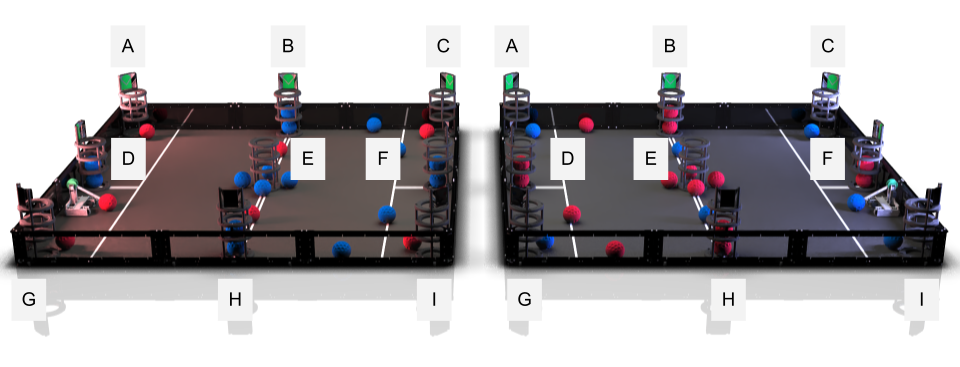
\includegraphics[scale=0.5]{labels}
\end{center}

\end{itemize}

\newpage

\section{Tournament Rules}

\begin{itemize}[label={}]
\item\textbf{$<$ORCAH-TR1$>$ Camera Setup} - Teams will be given the benefit of the doubt if all of these points cannot be reached.  We understand that it is difficult to fit a field and a correct camera setup in our homes.  Labeling the goals makes it easier for us to communicate with or without a proper camera setup.
\begin{itemize}
\item[--] Camera must be audience point of view and see the entire field
\item[--] Camera is tolerable +/- 40 degrees
\item[--] All goals must be labeled ABCDEFGHI
\item[--] Must be at least 720p
\end{itemize}

\item\textbf{$<$ORCAH-TR2$>$ 1 versus 1} - Matches will be played 1v1 with no alliance partner. 

\item\textbf{$<$ORCAH-TR3$>$ Elimination} - Eliminations will be a double elimination bracket.  Double eliminations is like a normal eliminations bracket, but with a second chance for teams that have lost their first eliminations match. \href{https://en.wikipedia.org/wiki/Double-elimination_tournament}{More information on how double eliminations work can be found here.}

\begin{itemize}
\item[--] Quarter-finals (and matches before) will be best of one (1).
\item[--] Semi-finals will be best of three (3).
\item[--] Finals will be best of five (5), where the winner of the upper bracket will start with an automatic one (1) win lead.
\end{itemize}

\item\textbf{$<$ORCAH-TR4$>$ For Teams Sharing a Field} - All teams sharing a field will be required to complete the Head Referee Certification.  Matches will be played using the VEX Game Manual and REC Foundation Q\&A except for the following:
\begin{itemize}
\item[--] Matches will be played as 1v1 instead of 2v2
\end{itemize}


\item\textbf{$<$ORCAH-TR5$>$ Competition Switch} - During matches, your controller must be plugged into a competition switch.  A drive team member must:
\begin{itemize}
\item[--] Keep track of time
\item[--] Enable/disable the competition switch at the appropriate times.
\end{itemize}

A referee will start a timer when your robot first moves.  If your robot is still moving past the allotted Driver Period and Autonomous Period times, a disqualification will be up to the Head Referee’s discretion. 

This rule is in place as an attempt to minimize the effects of video latency between teams and the event console.

\item\textbf{$<$ORCAH-TR6$>$ Software} - An event console is being developed for use in matches. More information and rules will come in a future update.

\item\textbf{$<$ORCAH-TR7$>$ Tournament Rankings} - Rankings during qualification rounds will be determined in the following order:

\begin{itemize}
\item[--] Win Points (WP)
\item[--] Autonomous Points (AP)
\item[--] Competition Skills Ranking (CSR)
\item[--] Electronic Tiebreaker
\end{itemize}

\end{itemize}

\section{Skills}

\begin{itemize}[label={}]

\item\textbf{$<$ORCAH-S1$>$ Tournament and Global Ranking} - Skills will be ranked the same for Global and Tournament rankings.  Rankings will happen in this order:

\begin{enumerate}
\item Robot Skills Score
\item Programming Skills Score
\item Programming Skills Stop Time
\item Driver Skills Stop Time
\item Programming Skills Attempts
\item Driver Skills Attempts
\item Second Highest Programming Skills
\item Second Highest Programming Skills Stop Time
\item Second Highest Driver Skills
\item Second Highest Driving Skills Stop Time
\item Third Highest Programming Skills
\item Third Highest Programming Skills Stop Time
\item Third Highest Driver Skills
\item Third Highest Driving Skills Stop Time
\end{enumerate}

\end{itemize}

\newpage

\section*{Changelog}
To submit feedback, please submit a form on the Q\&A page of the ORCAH website, or email us at orcah.robotics@gmail.com.

\vspace{0.25in}

\noindent
\textbf{v1.0.0}

\begin{itemize}
\item[--] First Release.
\end{itemize}

\noindent
\textbf{v1.1.0}

\begin{itemize}
\item[--] TR3 changed to include best of 1 semi-finals.
\item[--] Clarified $<$ORCAH-TR4$>$.
\item[--] Added $<$ORCAH-TR7$>$.
\item[--] Added the skills section and $<$ORCAH-S1$>$.
\item[--] Fixed typo on 2pt ball
\end{itemize}


\end{document}